\section{电流的效应}\label{sec:7-6}

导体中有没有电流,看不见也听不着,那么怎么才能知道呢?这个似乎不好解决的问题其实是很容易解决的。
原来,导体中有电流的时候,会发生一些特有的现象,根据这些现象就可以判定电流的存在。
我们把导体中有电流的时候发生的现象,叫做电流的效应。

电灯泡里的灯丝通过电流发光的时候,用手摸摸灯泡,可以觉得它比不发光的时候热。
从实验知道,一切导体,有电流通过的时候,都要发热。
\CJKunderwave{任何导体中有电流的时候,导体都要发热,这种现象叫做电流的热效应}。
电炉、电烙铁都是利用电流的热效应来工作的。

把两根碳棒立在盛着硫酸铜溶液的玻璃杯里,用导线把两根碳棒分别跟电池的两极连接起来(图 \ref{fig:7-15}),
在硫酸溶液中就有了电流,过几分钟后,跟负极相连的碳棒上出现一层红色的铜,这层铜是从硫酸铜溶液里分解出来的。
可见,\CJKunderwave{在导电的溶液里有电流的时候,溶液里要发生化学变化,这种现象叫做电流的化学效应}。
工业上利用电流的化学效应来提炼铝、铜等金属,以及在容易生锈的金属物品上镀一层防锈的金属。

\begin{figure}[htbp]
    \centering
    \begin{minipage}{7cm}
    \centering
    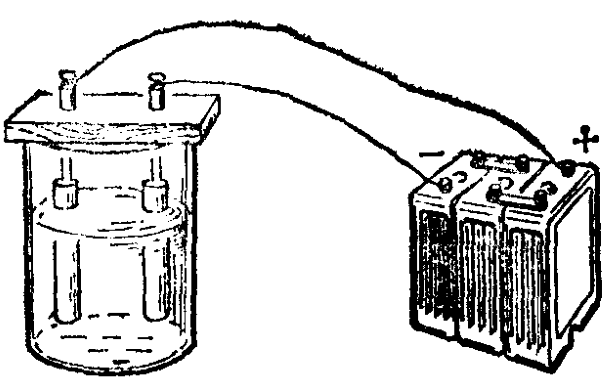
\includegraphics[width=6cm]{../pic/czwl2-ch7-15}
    \caption{}\label{fig:7-15}
    \end{minipage}
    \qquad
    \begin{minipage}{7cm}
    \centering
    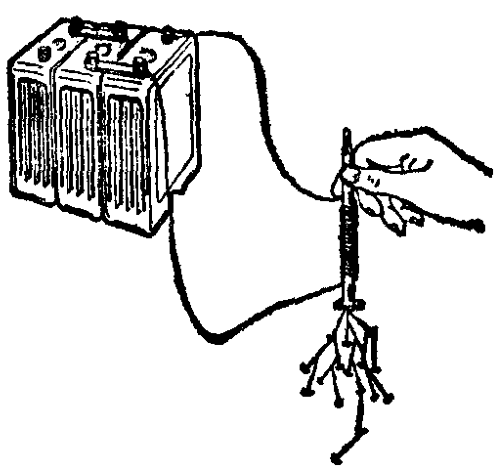
\includegraphics[width=6cm]{../pic/czwl2-ch7-16}
    \caption{}\label{fig:7-16}
    \end{minipage}
\end{figure}

在图 \ref{fig:7-16} 所示的实验中,把绝缘导线缠在一根铁钉上,当有电流通过时,铁钉能够吸引轻小的铁质东西如大头针、铁屑等,
表明铁钉变成了磁铁。电流一停止流通,被吸的东西就掉下来。
可见,\CJKunderwave{当导线中有电流的时候,在导线周围就产生跟磁铁相同的作用,这种现象叫做电流的磁效应}。

电流的各种效应,不但能使我们觉察电流的存在,而且使电流在许多方面获得了广泛的应用。
我们在这一节里只是初步提到某些应用,在后面还要继续学习。


\lianxi

(1) 在图 \ref{fig:7-17} 里,导线(或灯泡)中的电流方向是从锌筒到碳棒,还是从碳棒到锌筒?自由电子定向移动的方向呢?

\begin{figure}[htbp]
    \centering
    \begin{minipage}{7cm}
    \centering
    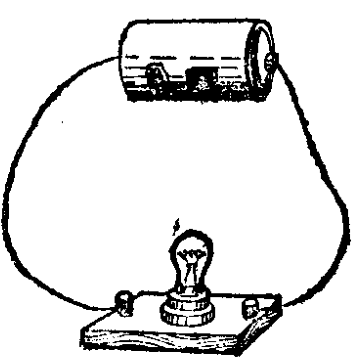
\includegraphics[width=4cm]{../pic/czwl2-ch7-17}
    \caption{}\label{fig:7-17}
    \end{minipage}
    \qquad
    \begin{minipage}{7cm}
    \centering
    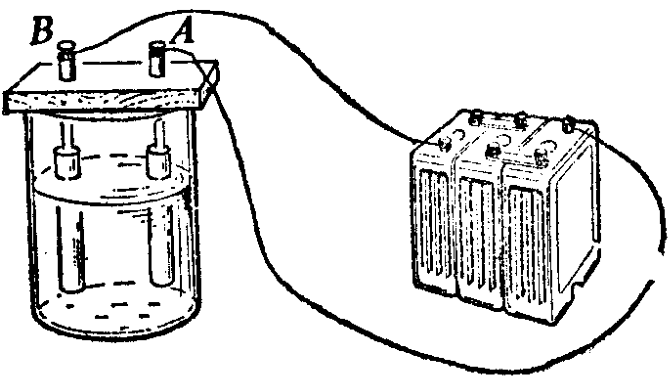
\includegraphics[width=6cm]{../pic/czwl2-ch7-18}
    \caption{}\label{fig:7-18}
    \end{minipage}
\end{figure}

(2) 在图 \ref{fig:7-18} 所示的装置里,碳棒 $A$、$B$ 立在硫酸铜溶液里,通电以后在碳棒 $A$ 上出现了一层红色的铜。
能不能根据这个现象确定电源的正、负极?在图中标出电流的方向。

\begin{figure}[htbp]
    \centering
    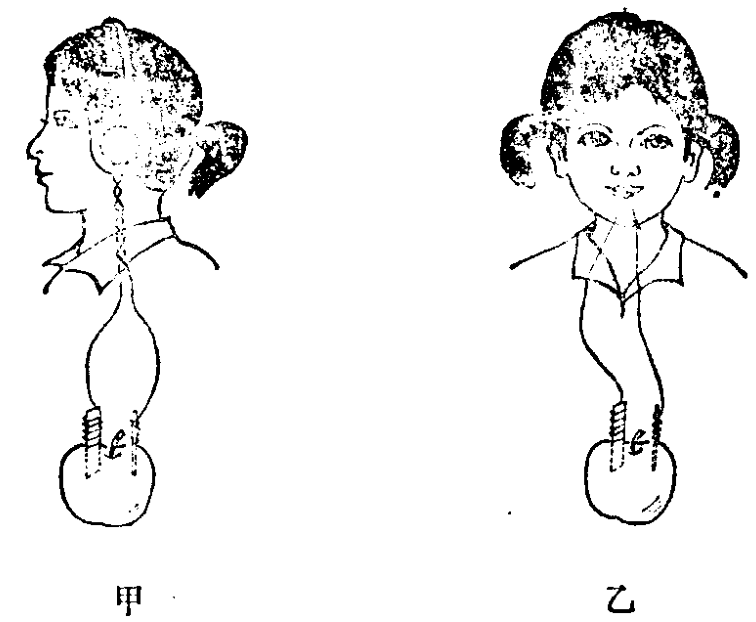
\includegraphics[width=0.6\textwidth]{../pic/czwl2-ch7-19}
    \caption{}\label{fig:7-19}
\end{figure}

(3) 做一个水果电池:找一根 5 厘米长的铜片或粗铜丝(也可以用绞在一起的几根细铜丝来代替),
再从废干电池上剪一条 2 毫米宽的锌皮,刮净,把铜丝和锌皮插入苹果或别的水果(也可以用番茄或土豆)里,
就做成了一个水果电池。将耳机线一根的末端接到一个电极上,当另一根的末端跟另一个电极断续接触时(图 \ref{fig:7-19} 甲),
从耳机里能听到电流引起的喀拉喀拉的声音。
也可以取两根导线,把它们的一端分别接到水果电池的两极,另一端和舌头断续接触(图 \ref{fig:7-19} 乙),
注意两根导线不要碰着,这时舌头上有什么异样的感觉?

